\chapter{Exam II (Practice)}
\label{ch:examii-practice}

\begin{preamble}
\begin{itemize}
\item You have 80 minutes to complete this examination.
\item Please answer all questions in the space provided with the
  question.  Clearly indicate your answers.
%% \item There are scratch pages at the end of the exam for your use. In no
%%   circumstance will anything you write on these pages count for or against
%%   your score on this exam.
\item You may refer to your one double-sided $8\frac{1}{2} \times 11$in
  sheet of paper with notes, but to no other person or source, during the
  examination.

\item Your answers for this exam must be written in blue or black ink.

\end{itemize}
\end{preamble}


\section{Problem 1: True or False}
%\newpage
%\input{truefalse}



\section{Problem 2: Short Answers}

%\input{../../../setstables/classes}
\begin{problem}[4pts][Classes]
\used{Fall 14, Final}

Lets say you are given a table that maps every student to the set of
classes they take.  

\ask
Fill in the algorithm below that returns all classes,
assuming there is at least one student in each class.  Your algorithm
must run in $O(m \log n)$ work and $O((\log m)(\log n))$ span, where
$n$ is the number of students and $m$ is the sum of the number of
classes taken across all students.    Note, our solution is one line.

\begin{lstlisting}[numbers=none]
fun allClasses($T$ : classSet studentTable) : classSet = 
@\vspace{.5in}@
\end{lstlisting}

\sol
\begin{lstlisting}[numbers=none]
fun allClasses($T$) = Table.reduce Set.union $\emptyset$ $T$
\end{lstlisting}
\end{problem}

%\input{../../../bfs/shortest-weighted}

\begin{problem}[5pts][Shortest Weighted]
\used{Fall 14, Practice Exam II}

Given a graph with integer edge weights between $1$ and $5$
(inclusive), you want to find the shortest \emph{weighted} path
between a pair of vertices. 

\ask
How would you reduce this problem to the
shortest \emph{unweighted} path problem, which can be solved using
BFS?

\sol
Replace each edge with weight $i$ with a simple path of $i$ edges
each with weight $1$. Then solve with BFS.
\end{problem}

%\newpage
%\input{../../../dfs/enterExit}
\begin{problem}[5pts][Enter and Exit]
 \used{Fall 14, Practice Exam II}

Recall the implementation of DFS shown in class using the \sml{enter}
and \sml{exit} functions. Circle the correct answer for each of the
following statements, assuming DFS starts at $A$:

\begin{center}
  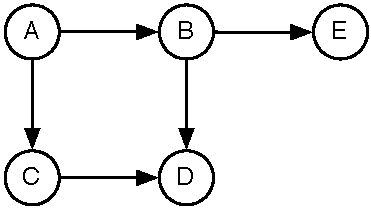
\includegraphics[scale=.7]{dfs/dfs-graph1.pdf}
\end{center}

\bigskip
  \begin{tabular}{lp{1.3in}cc}
    \texttt{enter D} could be called before \texttt{enter E}:& &
    \textsf{True} & \textsf{False}\\[1.5 ex]
    \texttt{enter E} could be called before \texttt{enter D}:& & \textsf{True} & \textsf{False}\\[1.5 ex]
    \texttt{enter D} could be called before \texttt{enter C}:& & \textsf{True} & \textsf{False}\\[1.5 ex]
    \texttt{exit A} could be called before \texttt{exit B}: & & \textsf{True} & \textsf{False}\\[1.5 ex]
    \texttt{exit D} could be called before \texttt{enter B}:&  & \textsf{True} & \textsf{False}
  \end{tabular}

\sol
    True, True, True, False, True
\end{problem}

%\input{../../../shortest-paths/fastroute}

\begin{problem}[5pts]
\used{Fall 14, Practice Exam II}

A new startup \emph{FastRoute} wants to route information along a path
in a communication network, represented as a graph. Each vertex
represents a router and each edge a wire between routers. The wires
are weighted by the maximum bandwidth they can
support. \emph{FastRoute} comes to you and asks you to develop an
algorithm to find the path with maximum bandwidth from any source $s$
to any destination $t$. As you would expect, the \emph{bandwidth} of a
path is the minimum of the bandwidths of the edges on that path; the
minimum edge is the \emph{bottleneck}.

\ask
Explain how to modify Dijkstra's algorithm to do this. In particular, how would
you change the priority queue and the following relax step?

\begin{quote}
\sml{fun relax (Q, (u,v,w)) = PQ.insert (d(u) + w, v) Q}
\end{quote}

Justify your answer.

\sol
  We'll use a max priority queue instead of a min priority queue used
  in Dijkstra's. We will also modify the relax step to insert into the
  priority queue $\min(d(u), w)$ because the quality of a path is the
  minimum of the edge weights. These changes don't affect the
  correctness of Dijkstra's, so we could explore the vertices like in
  Dijkstra's.
\end{problem}


%\newpage
%\input{../../../graph-contraction/cycleDetect}

\begin{problem}[4pts][Parallel Cycle Detection]
\ask
Describe in words how you would as part of star contraction 
efficiently detect that an undirected graph has a cycle.  \textbf{No more than two sentences.}

\sol
If during star contraction we find any self edges not involved in
contraction itself then there is a cycle.   However,
we need to be careful not to remove duplicate edges, and only to
contract along a single duplicate edge.

-4 if claim detecting duplicate edges is sufficient.  It is not sufficient because you can contract duplicate edges at the same time\\
%
-2 if say detect self edge, but do not point out issue with duplicates.\\
%
0 for DFS, BFS, etc.
\end{problem}


%\input{../../../graph-contraction/starContract}
%
\begin{problem}[6pts][Star Contraction]
\ask
Circle \textbf{every} type of graph listed below for which star
contraction will reduce the number of \textbf{edges} by a constant
factor in expectation in every round until fully reduced (and hence
imply $O(|E|)$ total work).  You can assume redundant edges between
vertices are removed.\\

(a) a graph in which all vertices have degree at most 2\\
(b) a graph in which all vertices have degree at most 3\\
(c) a graph in which all vertices have degree $\sqrt{|V|}$\\
(d) a graph containing a single cycle (i.e. a forest with one additional edge)\\
(e) the complete graph (i.e. an edge between every pair of vertices)\\
(f) any graph (still circle others if relevant)\\

\sol
a, d, e
\end{problem}


\begin{problem}[DFS Edges]
%\newpage
%\input{../../../dfs/edgeTypes}

The following questions have to do with the four types of edges in
a depth first search (DFS): \textbf{tree edges}, \textbf{back edges},
\textbf{forward edges} and \textbf{cross edges}.  For each one list
\textbf{all} types of edges that apply.


\ask [3]
What kind of edges can a \textbf{bridge}, as defined in AbridgedLab, be
\sol
tree edge

\ask [3]
Assume we enter $u$ before entering $v$ during the DFS, what kind of
edge can the edge $(u,v)$ (directed from $u$ to $v$) be?
\sol
forward edge, tree edge


\ask [3]
What kind of edges can appear in DFS for a directed graph in which
every edge appears in both directions (i.e. if $(u,v) \in E$ then $(v,u)
\in E$).
\sol
tree edges, forward edges, backward edges


\ask [3] Lets say that in a directed graph $u$ and $v$ are in two
different strongly connected components (in a strongly connected
component all vertices can reach all others).  What kind of edges can
be between $u$ and $v$.
\sol
tree edges, forward edges, cross edges

\ask [3]
In the topological sorting algorithm for directed acyclic graph we
described in class and the notes, lets say a vertex $u$ appears
after a vertex $v$.  What kind of edges can be in a path
from $v$ to $u$.
\sol
tree edges, forward edges, cross edges

\end{problem}


\section{Problem 3: Sets and Tables}


%\newpage
\section{(Sets and Tables) Bingled}


%\input{../../../setstables/bingled}

After forming your company Bingle to index the web allowing word
searches based on logical combination of terms (e.g. ``big'' and
``small''), you discover that there are already a couple companies out
there that do it....and lo-and-behold, they even have similar names.
You therefore decide to extend yours with additional features.  In
particular you want to support phrase queries: e.g. find all
documents where ``fun algorithms'' appears.

You decide the right way to represent the index is as a table of sets
where the keys of the table are strings (i.e. the words) and the
elements of the sets are pairs of values consisting of a document
identifier and an integer location in the document where the string
appears.  So, for example the following collection of three documents
with integer document identifiers:

\begin{quote}
\begin{tabbing}
 $\langle$
  \=(1, \ctext{``the big dog''}), \\
  \>(2, \ctext{``a big dog ate a hat''}),\\
  \>(3, \ctext{``i read a big book''}) $\rangle$
\end{tabbing}
\end{quote}

the document index would be represented as
\[
\begin{array}{ll}
\text{idx} = \{ & \ctext{``a''} \mapsto \cset{(2,0),(2,4),(3,2)}
\\
                &  \ctext{``big''} \mapsto \cset{(1,1),(2,1),(3,3)},
\\
                & \ctext{``dog''} \mapsto \cset{(1,2),(2,2)},
\\
                & \ldots
\\
             \} &
\end{array}
\]

In particular you want to support the following interface
\begin{lstlisting}[numbers=none]
signature INDEX = sig
  type word = string
  type docId = int
  type index = docIdIntSet wordTable
  
  (* represents all documents and all locations where a phrase appears *)
  type docList

  val makeIndex : (docId * string) seq -> index    
  val find : index -> word -> docList
  val adj : docList * docList -> docList
  val toSeq : docList -> docId seq 
end
\end{lstlisting}
%
where, given an index \sml{I},
\texttt{toSeq (adj (find I "210", find I "rocks"))} would return a sequence of
identifiers of documents
where ``210'' appears immediately before ``rocks'', and 
\\
\sml{toSeq (adj (find I "Umut", adj (find I "loves", find I "climbing")))}
\\
would return a sequence of identifiers of documents
where the phrase ``Umut loves climbing'' appears.


\begin{problem}[8p]
\ask
Show SML code to generate the index from the sequence of documents.
It should not be more than 8 lines of code and assuming all words have
length less than some constant, must run in $O(n \log n)$ work and
$O(\log^2 n)$ span, where $n$ is the total number of words across all
documents.    You can use a function
\begin{lstlisting}
val toWords~:~string -> string seq
\end{lstlisting}
that breaks a text string into a sequence of words.

\begin{lstlisting}[numbers=none]
type index = docIdIntSet wordTable

fun makeIndex (docs : (docId  * string) seq) : index =
  let
\end{lstlisting}

\sol

\begin{lstlisting} [numbers=none]
  fun tagWords (id,doc) = 
      let val words = toWords doc
      in  Seq.tabulate (fn i = (nth i words, (id, i)) (length words) 
      end

  val allPairs = Seq.flatten (Seq.map tagWords docs)

  val wordTable = Table.collect allPairs
in
    Table.map Set.fromSeq wordTable
end
\end{lstlisting}
\end{problem}

\begin{problem}[8p]

% Show code for a function \texttt{adj(docList1, docList2)} that given
% two docLists returns a docList in which those two words
% are adjacent.  For example for the index generated from the documents
% above, 
% \begin{quote}
% \texttt{toSeq(adj(find idx "a", find idx "big"))} 
% \end{quote}
% would return
% $\cseq{2, 3}$.  For full credit \texttt{adj} must be an associative operator.

\ask
Define the \sml{docList} type and implement the function \sml{adj} as defined above.
You might find the function \sml{setmap} useful. The solution should
only be a few lines of code.
\begin{lstlisting}[numbers=none]
fun setmap f s = Set.fromSeq (Seq.map f (Set.toSeq s)) 
\end{lstlisting}


\begin{lstlisting}[numbers=none]

type docList = 

fun adj (                ,               ) : docList =

\end{lstlisting}


\sol
\begin{lstlisting}[numbers=none]
type docList = (docIdIntSet)*int

fun adj ((d1,l1), (d2,l2)) = 
  let 
      val d2' = setmap (fn (d,i) = (d, i-l1)) d2
  in  
      (Set.intersection (d1,d2'), l1+l2)
  end

(* FYI: not part of exam *)
fun find idx word = 
  case Table.find idx word =>
    NONE => (Set.empty(), 1)
  | SOME d => (d, 1)
\end{lstlisting}
   
\end{problem}



%\newpage
\section{(Shortest Paths) Dijkstra and A*}
%\input{../../../shortest-paths/dijkstra-astar}

\used{Fall 14, Practice Exam II}

\begin{problem}[6pts]

Consider the graph shown below, where the edge weights appear next to
the edges and the heuristic distances to vertex $G$ are in parenthesis
next to the vertices.
\begin{center}
  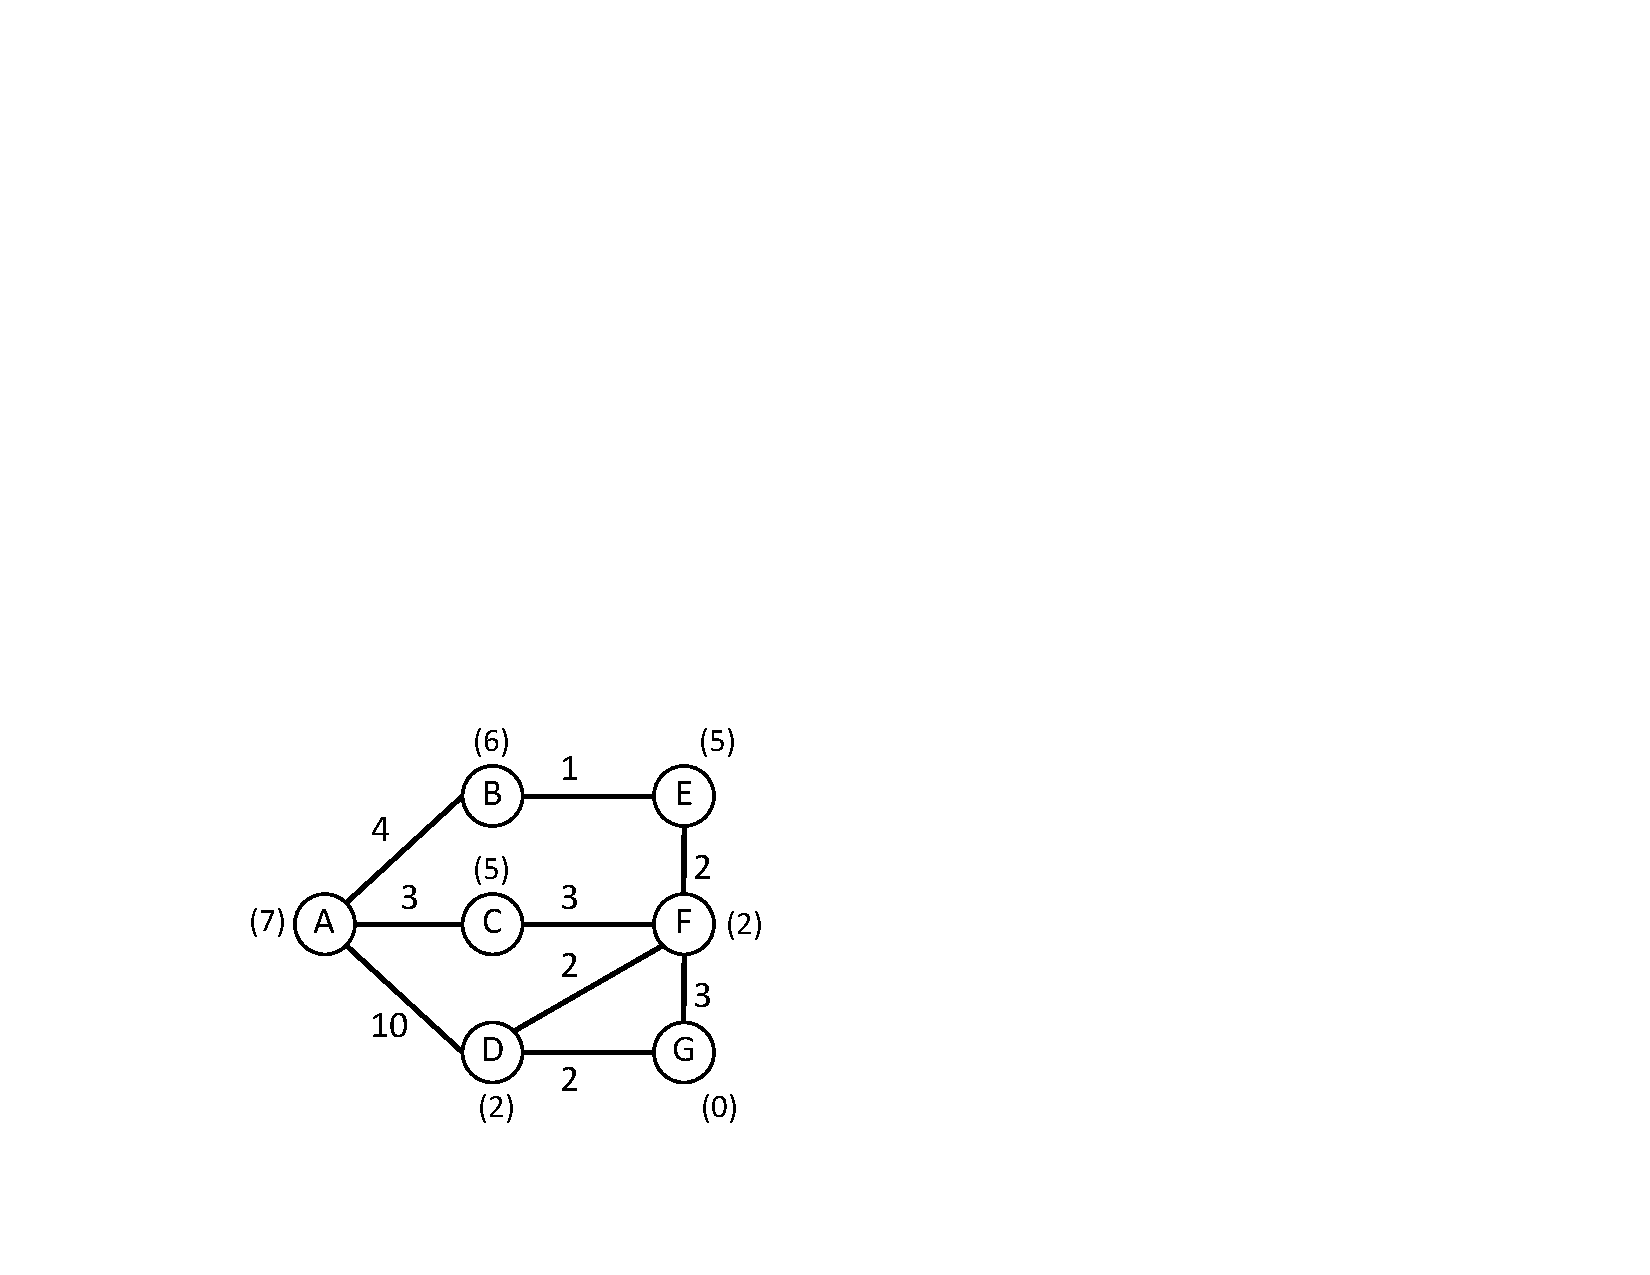
\includegraphics[scale=.75]{shortest-paths/graph.pdf}
\end{center}

\ask
Show the order in which vertices are visited by Dijkstra when the source
vertex is $A$.
\sol
A C B E F D G


\ask Show an order in which vertices are visited by $A^*$ when
the source vertex is $A$ and the destination vertex is $G$.

\sol
A C F G 

\end{problem}

\begin{problem}[4pts]

\ask
What is the key reason you would choose to use $A^*$ instead of
Dijkstra's algorithm?

\sol
You can use $A^*$ if you want the shortest path to only a single goal vertex,
and not all shortest paths. $A^*$ can be much more efficient, as it tries to
move toward the goal more directly, skipping many more vertices.
\end{problem}

\begin{problem}[5pts]
\ask
Show a $3$-vertex example of a graph on which Dijkstra's algorithm always
fails. Please clearly identify which vertex is the source.

\sol
\begin{verbatim}
         A 
        / \
   x=4 /   \ y=-2   x+y < z < x guarantees failure
      /     \       x+y < z <= x may fail depending on the input order
    S ------- B
        z=3
\end{verbatim}
\end{problem}


\section[12]{(Shortest Paths) Wormholes}

%\newpage
%\input{../../../shortest-paths/wormholes}


\used{Fall 14, Untested, needs some work}

In your new job for a secret Government agency you have been told
about the existence of wormholes (also known as Einstein-Rosen
bridges) that connect various locations in the country.  You have been
tasked with designing an algorithm for finding the shortest path using
a combination of roads and wormholes between a pair of locations.
Traveling through a wormhole is instantaneous, for all practical
purposes, but it turns out that on a given trip someone can only go
through two wormholes otherwise they risk rearrangement of their
atomic structure.

\begin{problem}
The wormhole problem is therefore the weighted shortest path problem
(assuming non-negative edge weights) with the additional constraint
that (1) some edges are specially marked, and (2) a path can take at
most two of those edges.

\ask
You still have your Dijkstra code from 210.  You don't want to change
your code---after all you forgot how ML works---so you just want to
preprocess your graph so that a call to your code \sml{SP}$(s,t)$
returns the correct solution to the wormhole problem.  Explain how to
do this. \textbf{At most 5 sentences.}

\sol
Create three copies of the graph without the wormhole edges: copy 0,
copy 1, and copy 2.  Connect copy 0 with copy 1 with the wormhole
edges, with weight 0.  Likewise connect copy 1 with copy 2 with
wormhole edges with weight 0.  Now find the shortest path from
\sml{SP}$(s,d)$ by starting at $s$ in copy 0 and finding the shortest
path to $d$ in any of the three copies.
\end{problem}



\section[10]{(Graphs) Strongly Connected Components}
\used{Fall 14, Practice Exam II}

%\newpage
%\input{../../../graphs/scc2}

A \emph{strongly connected component} of a directed graph $G = (V,E)$ is a subset $S$ of $V$ such
that every vertex $u \in S$ can reach every other vertex $v \in S$ (i.e.,
there is a directed path from $u$ to $v$), and such that no other vertex in
$V$ can be added to $S$ without violating this condition. Every vertex
belongs to exactly one strongly connected component in a graph.

\begin{problem}
\ask
Implement the function:
\begin{lstlisting}
val scc~:~graph * vertex -> vertexSet
\end{lstlisting}
such that \sml{scc(G,v)} returns the strongly connected component containing $v$. You may assume
the existence of a function:
\begin{lstlisting}
val reachable~:~graph * vertex -> vertexSet
\end{lstlisting}
such that \sml{reachable(G,v)} returns all the vertices reachable from $v$
in $G$, and 
\begin{lstlisting}
val transpose~:~graph -> graph
\end{lstlisting}
That takes every edge in a directed graph and reverses its direction.
You may assume the following representation of graphs:
\begin{lstlisting}
type graph = vertexSet vertexTable
\end{lstlisting}
with key comparisons taking $O(1)$ work.

Assuming that \texttt{reachable} and \texttt{transpose} use
$O(|E|\log|V|)$ work and $O(\log^2 |V|)$ span, your algorithm
must also have $O(|E|\log|V|)$ work and $O(\log^2 |V|)$ span.

\begin{lstlisting}[numbers=none]
fun scc ($G$ : graph, v : vertex) : vertexSet = @\vspace{.2in}@
      @\underline{~~~~~~~~~~~~~~~~~~~~~~~~~~~~~~~~~~~~~~~~~~~~~~~~~~~~~}@@\vspace{.2in}@
      @\underline{~~~~~~~~~~~~~~~~~~~~~~~~~~~~~~~~~~~~~~~~~~~~~~~~~~~~~}@
\end{lstlisting}


\sol
\begin{lstlisting}[numbers=none]
fun scc ($G$ : graph, v : vertex) : vertexSet = @\vspace{.2in}@
    @\underline{vertexSet.intersection(reachable(G,v),~~~~~~~~~~~~~}@@\vspace{.2in}@
    @\underline{~~~~~~~~~~~~~~~~~~~~~~~reachable(transpose(G,v)))}@
\end{lstlisting}

\end{problem}

